
\documentclass[a4paper]{report}
% \documentclass{report}
\usepackage[utf8]{inputenc}
\usepackage{amsmath}
\usepackage{esint}
\usepackage{tabstackengine}
\usepackage[colorlinks,linkcolor=blue]{hyperref}
\usepackage{xeCJK}
\usepackage{caption}
\usepackage{stackengine}
\usepackage{graphicx}
\graphicspath{ {../resources/figure/comm/} }
\usepackage{float}
\usepackage{amsmath}
\usepackage{ulem}
\usepackage{amsfonts}
\usepackage{blkarray}
\usepackage{enumitem}
\setlist[1]{itemsep=-5pt}
\usepackage{subcaption}
\usepackage{multirow}
\usepackage{tikz}
\usetikzlibrary{calc}
\usepackage{pgfplots}
\usepackage{mathrsfs}
\usepackage{minted}
\usepackage{booktabs}
\usetikzlibrary{shapes,arrows,positioning}
\captionsetup[table]{skip=10pt}

%%%% 下面的命令重定义页面边距,使其符合中文刊物习惯 %%%%
\addtolength{\topmargin}{-54pt}
\setlength{\oddsidemargin}{0.63cm}  % 3.17cm - 1 inch
\setlength{\evensidemargin}{\oddsidemargin}
\setlength{\textwidth}{14.66cm}
\setlength{\textheight}{24.00cm}    % 24.62


% 段首不缩进
\setlength{\parindent}{0pt}
%%%% 下面的命令设置行间距与段落间距 %%%%
\linespread{1.2}
% \setlength{\parskip}{1ex}
\setlength{\parskip}{.5\baselineskip}

\def\rlwd{.5pt} \def\rlht{2.2ex} \def\rldp{.5ex}
\def\mydiv#1{~%
  \rule[-\rldp]{\rlwd}{\rlht}%
  \setbox0=\hbox{~#1}%
  \stackunder[\dimexpr\rldp-\rlwd]{~#1}{\rule{\wd0}{\rlwd}}%
}

\title{comm_principle}
\author{Crosstyan}
\date{Dec 2020}


\begin{document}
\chapter{Introduction}
对应第一章绪论

是否是数字信号是看是否被量化, 而非是看是否取样. 

对比Discrete Time和Continuous 信号. 
\section{评价通讯系统}
\subsection{有效性}
\subsubsection{码元速率}
波特, 码元每秒. 
\begin{equation}
  R_B=\frac{1}{T_B}
\end{equation}
码元速率仅仅与码元宽度有关
\subsubsection{比特率}
二进制时和波特相同. 比特率总是大一些的, 是波特乘上信源熵. 
\begin{equation}
  R_b=R_B\cdot H(\textbf{X})
\end{equation}
信源等概时, M进制. 
\begin{equation}
  R_b=R_B\cdot \log_2{M}
\end{equation}
\subsubsection{基带利用率}
单位频带内能达到的信息速率
\begin{equation}
  \eta=\frac{R_B}{B}
\end{equation}
单位为波特每赫兹 Baud/Hz
\begin{equation}
  \eta=\frac{R_b}{B}
\end{equation}
单位为比特每秒每赫兹 bps/Hz或者bit/(s$\cdot$Hz)
\subsection{可靠性}
\subsubsection{误码率}
码元数在传送总码元中所占比例
\begin{equation}
  P_e=\frac{\text{错误接收码元}}{\text{传输总码元}}
\end{equation}
\subsubsection{误比特率}
错误接受的比特数(信息量)在传送总比特数(信息量)中所占比例
\begin{equation}
  P_b=\frac{\text{错误接收比特}}{\text{传输总比特}}
\end{equation}
二进制时两者相等, 否则时误比特率大
\chapter{Deterministic Signal}

\section{确知信号的分类}
Periodic或者Nonperiodic信号. 

\subsection{能量与功率信号}
信号的能量
\begin{equation}
  E=\int_{-\infty}^\infty s^2(t)\;\text{d}t
\end{equation}
或者使用和功率类似的定义
\begin{equation}
  E=\lim_{T\rightarrow \infty}\int_{-\frac{T}{2}}^{\frac{T}{2}} s^2(t)\;\text{d}t
\end{equation}

$s^2(t)$为信号电压(电流)的瞬时时间波形. 单位为焦耳. 

而信号的平均功率的定义为
\begin{equation}
  P=\lim_{T\rightarrow \infty}\frac{1}{T}\cdot\int_{-\frac{T}{2}}^{\frac{T}{2}} s^2(t)\;\text{d}t
\end{equation}
常识告诉我们
\begin{equation}
  E=P\cdot t
\end{equation}
$t$为持续的时间. 

可以分类为
\begin{itemize}
  \item 有限能量, 零功率
  \item 无穷能量, 有限功率
  \item 无穷能量, 无穷功率
\end{itemize}
不存在零能量, 有限功率或者无穷功率. 或者有限能量, 无限功率; 因为$E=P\cdot t$, 能量绝对不能比功率小. 
\subsection{能量有限信号}
又被称作能量信号(Energy Signal); 有限能量, 平均功率绝对是零\footnote{$P=\displaystyle\lim_{T\rightarrow \infty}\frac{E}{T}$有限值除以无穷自然为零}. 

典型的信号是偶对称的信号. $t\rightarrow \infty$其值为零的信号. 

\textbf{所有有限数量脉冲都是能量信号}
\subsection{功率有限信号}
又被称作功率信号; 功率有限, 能量自然无限. \footnote{无穷除以无穷才可能等于常数} 
不带平方积分的话多半积分值为零? 这种感觉. 

典型信号为无限长的白噪声, 或者是无限延伸的正弦波. 

\textbf{所有周期信号都是功率信号} (有界的)
\subsection{非功非能信号}
无穷能量, 又无穷功率. 无限延伸, 无穷无尽. 什么正比例函数啥的都算. 
\section{频谱密度}
\subsection{能量信号}
非周期函数(能量信号)使用FT来分析. 
\begin{equation}
  S(\omega)=\int_{-\infty}^{\infty}s(t)\cdot e^{-j\omega t}\; \text{d}t
\end{equation}
门函数的FT就是Sa函数(Sampling function 采样函数), 又称sinc. 
\subsection{功率信号}
周期函数(功率信号)使用FS来分析. 引入冲激函数$\delta(t)$
% \begin{equation}
%   S(k)=\frac{1}{T}\cdot \int_{0}^{T}s(t)\cdot e^{j\frac{2\pi}{T}\cdot kt}\;\text{d}t
% \end{equation}
\section{能量信号的能量谱密度}
只有能量信号才能拥有能量谱密度(连续谱). 取模平方一下就好
\begin{equation}
  G(f)=\lvert S(f)\rvert^2
\end{equation}
单位为焦耳每赫兹
\section{功率信号的功率谱密度}
PSD; 功率信号才能拥有功率谱密度(离散谱). FS\footnote{CTFS是非周期信号啦}的系数取模平方一下就好
\begin{equation}
  P(f)=\displaystyle\sum_{n=-\infty}^{\infty}\lvert C_n\rvert^2
\end{equation}
单位为(信号单位\footnote{如电压, 电流等}的平方)每赫兹
\section{自相关函数}
\begin{equation}
  R(\tau)=E[\xi(t)\cdot \xi(t+\tau)]
\end{equation}
维纳辛钦关系, 自相关函数和谱密度\footnote{功率谱密度(离散谱), 能量谱密度(连续谱). }为一对傅里叶变换. 
\begin{equation}
  E=R(0)
\end{equation}
自相关函数参数取值为0, 就等于能量. 




\chapter{Stochastic process}
对应通信原理第二章, 确定信号; 第三章, 随机过程. 
\section{随机过程}
\subsection{期望}
加权平均, 要求出$X$的分布率

若随机过程的PDF为$f(x,t)$, 则其期望为
\begin{equation}
  E[\xi(t)]=\int_{-\infty}^\infty x\cdot f(x,t)\;\text{d}t=a(t)
\end{equation}
\subsection{方差}
平方的期望减去期望的平方, 当然要求出$X^2$的分布率了
\begin{equation}
  D[X]=E[X^2]-E^2[X]
\end{equation}
\subsection{自相关}
衡量同一过程的不同时间的相关程度, 假设$\xi(t)$是一个随机过程
\begin{equation}
  R(t_1,t_2)=E[\xi(t_1)\xi(t_2)]
\end{equation}
\begin{equation}
  R(t_1,t_2)=\int_{-\infty}^\infty \int_{-\infty}^\infty x_1\cdot x_2\cdot f(x_1,x_2;t_1,t_2)\;\text{d}x_1 \text{d}x_2
\end{equation}
\subsection{互相关}
两个随机过程在不同时间的相关程度, 假设$\xi(t)$和$\eta(t)$是一个随机过程
\begin{equation}
  R(t_1,t_2)=E[\xi(t_1)\eta(t_2)]
\end{equation}
\section{Stationary}
平稳过程. 随机过程的统计特性与时间起点无关. 
\begin{itemize}
  \item 严平稳的一维PDF与时间$t$无关; 
  \item 严平稳的二维PDF只与时间间隔$\tau=t_2-t_1$有关
\end{itemize}
\subsection{广义平稳}
\begin{itemize}
  \item 广义平稳的期望与时间$t$无关; $E[\xi(t)]=\text{const}=a$
  \item 广义平稳的相关函数(自相关函数)只与时间间隔$\tau=t_2-t_1$有关 $R(t_1,t_1+\tau)=R(\tau)$
\end{itemize}
\subsection{平稳的数字特征}
若$\xi(t)$为Stationary, 则自相关函数$$R(t,t+\tau)=R(\tau)=E[\xi(t)\cdot\xi(t+\tau)]$$
\begin{itemize}
  \item 随机过程的平均功率 $R(0)=E[\xi^2(t)]$
  \item $R(\tau)$为偶函数
  \item $R(\tau)$的最大值为$R(0)$, 也就是说在$\tau=0$时有最大值
  \item $R(\infty)=E[\xi(t)]^2=a^2$表示随机过程的直流功率
  \item $R(0)-R(\infty)=\sigma^2$, $\sigma^2$为方差. 表示随机过程的交流功率. 当均值为0(直流功率为0)时, $R(0)=\sigma^2$
  \item $R(0)$为平稳过程的总功率. 
\end{itemize}
\subsection{Wiener–Khinchin theorem}
平稳过程的自相关函数$R(t,t+\tau)=R(\tau)$与其功率谱密度$P(f)$为一对傅里叶变换
\begin{equation}
  P_\xi(\omega)=\int_{-\infty}^\infty R(\tau)\cdot e^{-j\omega\tau}\;\text{d}\tau 
\end{equation}
\begin{equation}
  R(\tau)=\frac{1}{2\pi}\int_{-\infty}^\infty P_\xi(\omega)\cdot e^{j\omega\tau}\;\text{d}\omega 
\end{equation}
或者$\omega=2\pi f$改为线频率的表达式

$R(0)$为平稳过程的总功率. 

\section{Ergodicity}
各态历经性又称遍历性、埃尔哥得性。

若其「统计平均」与「时间平均」的数学期望和相关函数均相等, 则满足Ergodicity. 

时间平均的数学期望
\begin{equation}
  \bar{a}=\lim_{T\rightarrow\infty} \frac{1}{T}\int_{-\frac{T}{2}}^{\frac{T}{2}} x(t)\;\text{d}t
\end{equation}
时间平均的(自)相关函数
\begin{equation}
  \overline{R(\tau)}=\lim_{T\rightarrow\infty} \frac{1}{T}\int_{-\frac{T}{2}}^{\frac{T}{2}} x(t)\cdot x(t+\tau)\;\text{d}t
\end{equation}
\section{Gaussian Random Process}
\begin{itemize}
  \item (广义)平稳高斯过程也是严平稳的
  \item 高斯过程统计独立 $f_n(x_1,x_2\dots x_n;t_1,t_2\dots t_n)=\prod f(x_i;t_i)$
  \item 几个高斯过程的和, 也是高斯过程
  \item 高斯过程经过线性变换仍然是高斯过程
\end{itemize}
\subsection{高斯随机变量}
就是正态分布
\begin{equation}
  f(x)=\frac{1}{\sqrt{2\pi}\cdot\sigma}\cdot e^{-\frac{(x-a)^2}{2\cdot\sigma^2}}
\end{equation}
标准正态分布, $a=0,\;\sigma=1$
\subsection{各种性质}
期望
\begin{itemize}
  \item 参数为常数, 结果为常数
  \item 常数乘随机变量, 常数提出来
  \item 参数俩随机变量相加, 期望相加
  \item 俩随机变量相乘, 若独立, 期望相乘
\end{itemize}
方差
\begin{itemize}
  \item 常数的方差为0
  \item 常数乘随机变量, 提出来为常数的平方
  \item 常数加随机变量, 就等于随机变量的方差
  \item 随机变量独立时, 参数俩随机变量相加, 方差相加
\end{itemize}
\section{平稳过程通过线性系统}
\begin{equation}
  \xi_{\text{output}}(t)=h(t)*\xi_{\text{input}}(t)
\end{equation}
$*$ 为卷积
\subsection{输出的期望}
乘上$f=0$的频率响应, 也就是直流增益; 也就是$H(0)$
\begin{equation}
  E[\xi_o(t)]=E[\xi_i(t)]\cdot H(0)=\text{const}
\end{equation}
\subsection{输出的方差}
方差得通过自相关函数来求. 零时刻的自相关函数(总功率)减去无穷时刻的自相关函数(直流功率)(其差对应的是交流功率)
\begin{equation}
  \sigma^2=R_o(0)-R_o(\infty)
\end{equation}
\subsection{输出的自相关函数}
依然与起点无关, 但是表达式肯定和输入的不一样
$$R_o(t,t+\tau)=R_o(\tau)$$
满足维纳辛钦关系
\begin{equation}
  \text{FT}[R_o(t)]=P_o(\omega)
\end{equation}
\subsection{功率谱密度}
乘上频率响应的平方
\begin{equation}
  P_o(f)=\lvert H(f)\rvert^2\cdot P_i(f)
\end{equation}
满足维纳辛钦关系
\begin{equation}
  \text{IFT}[P_o(\omega)]=R_o(t)
\end{equation}
\section{白噪声}
该噪声的功率谱密度在所有频率上均为常数; 自相关函数为
\begin{equation}
  R(\tau)=\frac{n_0}{2}\cdot \delta(t)
\end{equation}
仅仅在$\tau=0$时才相关. 

过理想低通滤波器为低通白噪声, 过理想带通滤波器为带通白噪声. 
\chapter{Channel}
对应第四章, 信道
\section{视线传播距离}
地球是圆的, 天线是直的, 杵俩根杆子叫天线, 高度自然是一样的为$h$

天线高度与视线传输距离关系为
\begin{equation}
  h\approx \frac{D^2}{50}
\end{equation}
$D$的单位为千米, $h$的单位为米. 这只能拿来估算啦\dots
\begin{figure}[H]
\centering
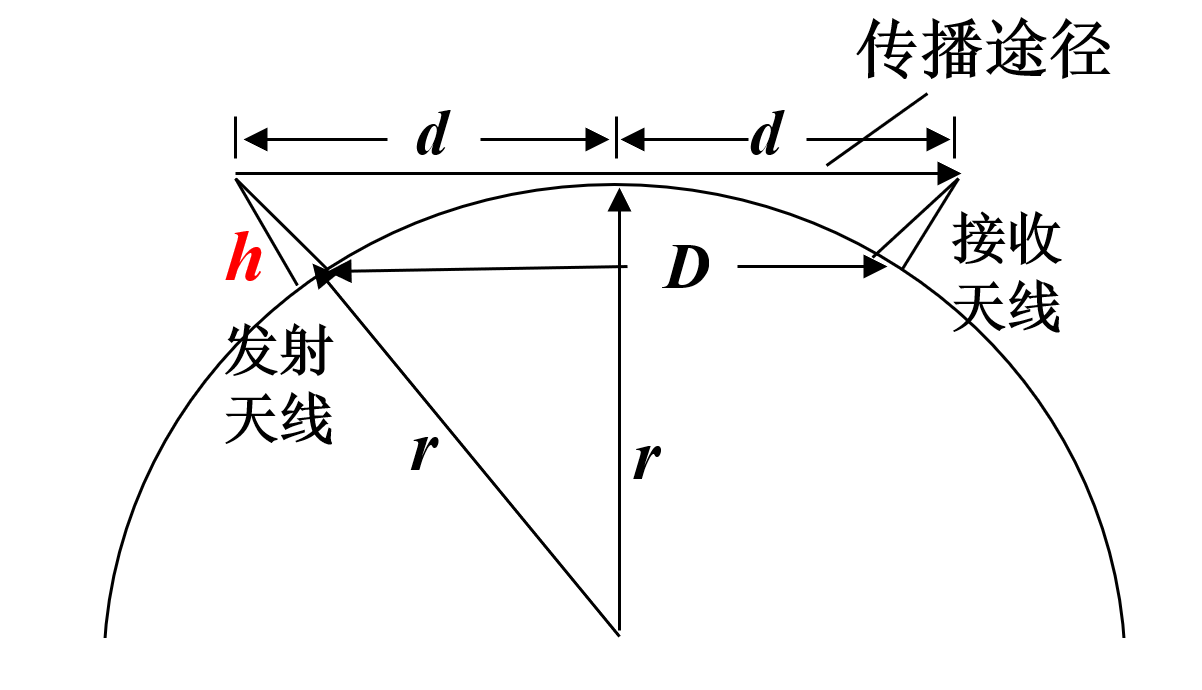
\includegraphics[width=0.5\textwidth]{dist.png}
\caption{视线传播模型}
\end{figure}
$h$为天线高度, $D$为两地的直接距离(横着地球切过来), $r$为地球半径, $d$为传播途径距离(与地球相切). 
可以易得
\begin{align*}
   D^2&\approx(2d)^2 \qquad\text{没有这个约等关系没法算}
  \\ \text{三角形中间那条腰的高度}&\approx r \qquad\text{没有这个约等关系没法算}
  \\ d^2+r^2&=(h+r)^2
\end{align*}
推导得到最终表达式
\begin{equation}
    (\frac{D}{2})^2+r^2=(h+r)^2
\end{equation}

\paragraph{天波传播}
若用电离层反射, 那就相当于拿电离层当天线, 其高度就是电离层高度. 这时候就不能估算了. 
\chapter{Source}
对应第十章, 信源编码
\chapter{Analog Passband Modulation}
对应第五章, 模拟调制系统. 相当于高频电子电路里面的调制. 
\section{AM}
\begin{equation}
  [1+m(t)]\cdot \text{Carrier}
\end{equation}
若用频率为$\omega_c$当载波
\begin{equation}
  [1+m(t)]\cdot A\cos{(\omega_c\cdot t)}
\end{equation}
假设被调波为$\cos(\omega_m\cdot t)$
\begin{align*}
  S_{AM}(\omega)=& \pi\cdot [\delta(\omega+\omega_c)+\delta(\omega-\omega_c)]&&\text{载波频率}
  \\ &+ \frac{1}{2}\cdot\pi\cdot [\delta(\omega-\omega_c-\omega_m)+\delta(\omega+\omega_c+\omega_m)]&&\text{上边频}
  \\ &+ \frac{1}{2}\cdot\pi\cdot [\delta(\omega+\omega_c-\omega_m)+\delta(\omega-\omega_c+\omega_m)]&&\text{下边频}
\end{align*}
DSB/SC没有载波频率; SSB/SC只有上边频/下边频;

调制度$m_a$
\begin{equation}
  m_a=\frac{\text{待调波形振幅}}{\text{载波波形振幅}}
\end{equation}
\subsection{抗噪性能}
DSB和SSB的输出噪声都会减少$\frac{1}{4}$
\section{FM}
$f_m$指被调波的最大频率
\begin{align*}
    v_c(t)&=V_c\cdot\cos(\omega_c\cdot t)
    \\ v_\Omega(t)&=V_\Omega\cdot\cos(\Omega t)=V_\Omega\cdot\cos(2\pi f_m\cdot t)
    \\ v_{\text{FM}}&=V_0\cdot\cos[\int_0^{t} f(t)\; \text{d}t]
    \\ f(t)&=\omega_c+k_f\cdot v_\Omega
    \\ \Delta f_m &= k_f\cdot \max[v_\Omega(t)]
\end{align*}
调频指数是最大相位偏移 (调相指数也是最大相位偏移)
\begin{equation}
  m_f=k_f\cdot \max[v_\Omega(t)]
\end{equation}
带宽
\begin{equation}
  2\cdot (m_f+1)\cdot f_m
\end{equation}
\section{制度增益}
制度增益\begin{equation}
  G=\frac{\text{SNR}_o}{\text{SNR}_i}
\end{equation}
表示调制后信噪比的改善. 

不能说明DSB系统的抗噪声性能优于SSB. 在相同条件下两者的输出信噪比是相等的. 
\section{系统比较}
所有系统在「同等条件下比较」
\begin{itemize}
  \item 解调器输入信号功率$S_i$
  \item 信道噪声均值为0, 单边功率谱密度为$n_0$
  \item 基带信号带宽为$f_m$
  \item AM的调幅度为$100\%$
\end{itemize}
% Table generated by Excel2LaTeX from sheet 'Sheet1'
\begin{table}[htbp]
  \centering
    \begin{tabular}{|c|ccc|}
    \toprule
    调制方式  & 信号带宽  & 输出信噪比 & 制度增益 \\
    AM    &   $2f_m$    &  $\frac{1}{3}\cdot \frac{S_i}{n_0\cdot f_m}$     & $\frac{2}{3}$ \\
    DSB   &    $2f_m$   &   $\frac{S_i}{n_0\cdot f_m}$    & 2 \\
    SSB   &     $f_m$  &    $\frac{S_i}{n_0\cdot f_m}$   & 1 \\
    VSB   &     略大$f_m$  &  近似SSB     & 近似SSB \\
    FM    &    $2(m_f+1)\cdot f_m$   &   $\frac{3}{2}\cdot m_f^2\cdot \frac{S_i}{n_0\cdot f_m}$    & $3m_f^2\cdot (m_f+1)$ \\
    \bottomrule
    \end{tabular}%
  \caption{各模拟调制性能比较}
\end{table}%
\paragraph{性能比较}
\begin{itemize}
  \item 抗噪声性能:FM最好,DSB/SSB、VSB次之,AM最差;
  \item 频谱利用率:SSB最高,VSB较高,DSB/AM次之,FM最差;
  \item 功率利用率:FM最高,DSB/SSB、VSB次之,AM最差;
  \item 设备复杂度:AM最简,DSB/ FM次之,VSB较复杂, SSB最复杂。
\end{itemize}
\paragraph{特点和应用}
\begin{itemize}
  \item AM:优点是接收设备简单;缺点是功率利用率低,抗干扰能力差。主要用在中波和短波调幅广播。
  \item DSB:优点是功率利用率高,带宽与AM相同。主要用于调频立体声中的差信号调制,彩色TV中的色差信号调制。
  \item SSB:优点是功率利用率和频带利用率都较高,抗干扰能力和抗选择性衰落能力均优于AM,而带宽只有AM的一半;缺点是收发设备都复杂。常用于频分多路复用系统中。
  \item VSB:抗噪声性能和频带利用率与SSB相当。在电视广播等系统中得到了广泛应用。
  \item FM: 抗干扰能力强,广泛应用于长距离高质量的通信系统中。缺点是频带利用率低,存在门限效应。
\end{itemize}
\chapter{Digital Baseband}
对应第六章, 数字基带传输系统
\section{数字基带传输系统构成}
\begin{figure}[H]
\centering
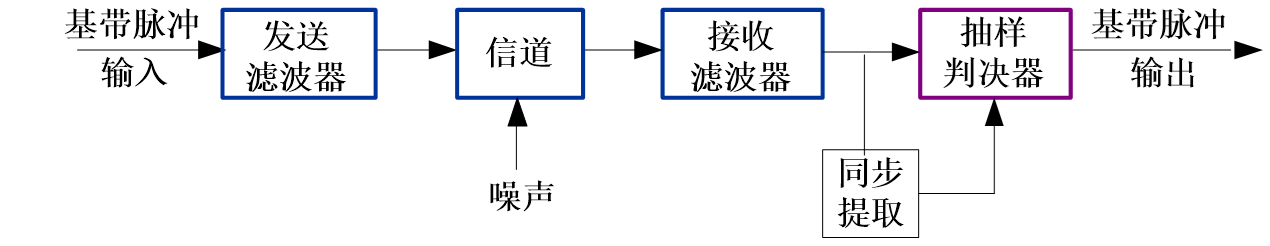
\includegraphics[width=0.7\textwidth]{baseband_system.png}
\caption{数字基带传输系统}
\end{figure}
\begin{itemize}
  \item 发送滤波器: 原始基带信号变为适合信道传输的基带信号; 目的为匹配信道, 减少码间串扰, 利于同步提取.
  \item 接收滤波器: 用于滤除带外噪声, 对信道特性均衡
  \item 抽样判决器: 对接收滤波器的输出波形进行抽样判决; 确定发送信码徐磊, 再生基带信号
  \item 同步提取: 提取用于抽样的位定位脉冲
\end{itemize}

\begin{itemize}
  \item 功率谱密度
  \item 无码间串扰 (Inter-Symbol Interference) 传输特性
  \item 部分响应
  \item 时域均衡
\end{itemize}
\section{基带信号分类}
\subsection{Return Zero}
\subsubsection{RZ}
信号电压在一个码元终止时刻总是会到零电平

占空比, $\tau$为信号电平的持续时间
\begin{align*}
  \frac{\tau}{T_B}=50\%
\end{align*}
\subsubsection{NRZ}
不归零编码 (non-return-to-zero line code, NRZ) 
\begin{align*}
  \frac{\tau}{T_B}=100\%
\end{align*}
\subsection{相对码 Differential}
以相邻脉冲电平的相对变化来表示消息
\subsection{多电平波形}
多个二进制码元对应一个脉冲
\section{基本信号波形}
\begin{figure}[H]
\centering
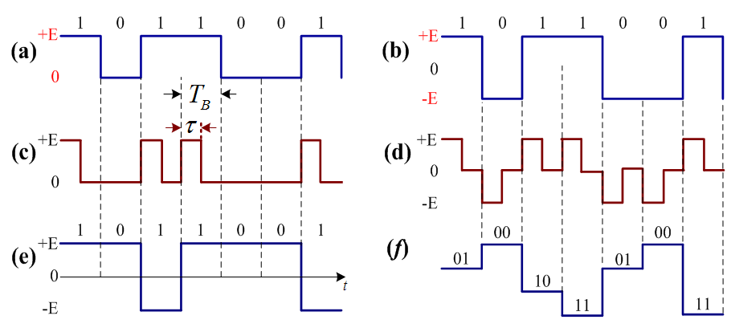
\includegraphics[width=0.8\textwidth]{baseband_signal.png}
\caption{基本信号波形}
\end{figure}
\begin{itemize}
  \item (a) 单极性NRZ
  \item (b) 双极性NRZ
  \item (c) 单极性RZ
  \item (d) 双极性RZ
  \item (e) 差分双极性NRZ
  \item (f) 多电平NRZ
\end{itemize}
\subsection{单极性波形}
NRZ, 绝对码. 有直流分量
\begin{itemize}
  \item 1为正电平
  \item 0为零电平
\end{itemize}
\subsection{双极性}
NRZ, 绝对码
\begin{itemize}
  \item 1为正电平
  \item 0为负电平
\end{itemize}
1和0等概出现时无直流分量
\subsection{单极性归零}
RZ, 绝对码

RZ可以直接提取定时信息
\subsection{双极性归零}
RZ, 绝对码

易于同步. 
\subsection{Differential}
NRZ, 双极性

相邻码元的电平的跳变和不变来表示信息
\begin{itemize}
  \item 1为电平跳变
  \item 0为电平不变
\end{itemize}
消除相位模糊
\subsubsection{传号差分}
1变0不变
\subsubsection{空号差分}
0变1不变
\subsection{多电平}
NRZ

比特率
\begin{align*}
  R_b=R_B\cdot \log_2{M}
\end{align*}
\section{常用的传输码型}
\subsection{AMI码}
Alternative Mark Inversion

将1交替变为+1和-1

优点: 没有直流成分, 高低频分量少, 全波整流变为单极性RZ码
\\缺点: 连续0时定时提取困难
\subsection{HDB3码}
High Density Bipolar of Order 3

\begin{itemize}
  \item 连0小于3和AMI相同
  \item 连0大于3, 每四个连0化为一组, 用$000V$替代; 极性与前一个非0脉冲极性相同, V为破坏脉冲
  \item 相邻V码极性必须交替, 若$000V$不满足条件则使用$B00V$来替代, B的取值与组内V脉冲一致, B被称作调节脉冲
\end{itemize}
\begin{minted}{javascript}
if(GetSerialZeros==4){
  Code=B+0+0+V;
  V.Polar=LastNonZeroCode.Polar;
  if(V==LastV){
    B.Polar= ~LastNonZeroCode.Polar;
    V.Polar=B.Polar;
  }else{
    B=0;
    // V.Polar=LastNonZeroCode.Polar;
  }
}
\end{minted}
有调节脉冲B出现之后, 连续出现的0应该都要有调节脉冲啦\dots (直到连续结束) 除了V位以外, 其他所有脉冲必须符合AMI码
\subsubsection{解码}
\begin{itemize}
  \item 找到破坏点V (极性非交替的大概就是1) 
  \item V及其前三个符号变成0
  \item 正负1变为1
\end{itemize}
\subsection{双向码/曼彻斯特码}
双极性RZ, 丰富的定时信息, 没有直流分量. 

0编码为01, 1编码为10 (带宽加倍)
\subsection{CMI码}
coded mark inversion
\begin{itemize}
  \item 1: 交替的11和00表示
  \item 0: 用01表示
\end{itemize}
\section{数字基带的频谱特性}
$a_n$为电平值, $T_B$为电平持续时间
\begin{align*}
  s(s)=\displaystyle\sum_{n=-\infty}^{\infty}a_n\cdot g(t-n\cdot T_B)
\end{align*}
其功率谱密度由稳态波$v(t)$和交变波$u(t)$构成
\begin{align*}
  P_s(f)=P_u(f)+P_v(f)
\end{align*}
假设
\begin{equation}
  \begin{cases}
    g_1(t-nT_B)&\text{概率为}P
    \\ g_2(t-nT_B)&\text{概率为}1-P
  \end{cases}
\end{equation}
仅记忆双边谱即可, $P$为其中一个符号出现概率, $1-P$则代表另一符号出现概率. $f_B=\frac{1}{T_B}$为码元速率, $T_B$为码元宽度. $G(f)$为$g(t)$的傅里叶变换. $m$表示该信号为直流或定时分量. 
\begin{align*}
  P_s(f)&=f_B\cdot P(1-P)\cdot\lvert G_1(f)-G_2(f)\rvert^2 &&\text{连续谱}
  \\ &+\displaystyle\sum_{m=-\infty}^{\infty}\lvert f_B\cdot [P\cdot G_1(mf_B)+(1-P)\cdot G_2(mf_B)]\rvert^2\cdot \delta(f-mf_B) &&\text{离散谱}
\end{align*}
\begin{equation}
  \begin{cases}
    m=0 &\text{直流分量}
    \\ m=\pm 1 &\text{定时分量}
  \end{cases}
\end{equation}

连续谱$f_B\cdot P(1-P)\cdot\lvert G_1(f)-G_2(f)\rvert^2$总是存在的, 而离散谱是否出在取决于$g(t)$和$P$, 当$g_1(t)=-g_2(t)$, 且$P=\frac{1}{2}$, 也就是双极性等概时, 离散谱不存在

\subsection{例题}
单极性码设$g_1(t)=0$, $g_2(t)=g(t)$, 那么$G_1(f)=0$, $G_2(f)=G(f)$. 

$g_2(t)=1$是不够有普适性的. 为了保持普适性$g_2(t)=g(t)$. 一般认为$P=1-P=\frac{1}{2}$等概. 

对于单极性NRZ
\begin{equation}
  g(t)=\begin{cases}
    1&\lvert t \rvert \leq \frac{T_B}{2}
    \\ 0 &\text{elsewhere}
  \end{cases}
\end{equation}
那么可以明确得到其傅里叶变换为
\begin{equation}
  G(f)=T_B\cdot \text{sinc}(\pi\cdot T_B \cdot f)
\end{equation}
其中
\begin{equation}
  \text{sinc}(x)=\frac{\sin{(x)}}{x}
\end{equation}
当$f=mf_B$时, 讨论离散谱是否存在, 也就是$m$的取值. 

对于单极性RZ时, $g(t)$占空比为50\%, 有
\begin{equation}
  G(f)=\frac{T_B}{2}\cdot \text{sinc}(\pi\cdot \frac{T_B}{2} \cdot f)
\end{equation}
结合$\text{sinc}(x)$函数的性质来讨论$m$的取值对$\text{sinc}(\pi \frac{T_B}{2}\cdot mf_B)$的影响

\paragraph{小结}
时域占空比越小, 占用频带越高. 
$$B_s=\frac{1}{\tau}=\begin{cases}
  f_B&\text{NRZ}_{\tau=T_B}
  \\ 2\cdot f_B&\text{RZ}_{\tau=\frac{\tau}{2}}
\end{cases}$$
\subsection{如何求功率}
知道双边功率谱密度之后就直接对$P_s(f)$在无限域上积分就好了. 
\begin{equation}
  P=\int_{-\infty}^{\infty}P_s(f)\;\text{d}f
\end{equation}
\subsection{三角波的FT}
$T$为门宽, $E$为门高
\begin{equation}
  G(f)=\underset{\text{三角形面积}}{\frac{ET}{2}}\cdot \text{sinc}(T \cdot\frac{1}{2}\cdot\frac{\omega}{2})
\end{equation}
\section{Inter-Symbol Interference}
无码间串扰 (Inter-Symbol Interference) 传输特性

误码
\begin{itemize}
  \item AWGN
  \item ISI 前一码元拖尾过长, 蔓延到当前码元的抽样时刻上
\end{itemize}
滤波器
\begin{itemize}
  \item $G_T(\omega)$ 发送滤波器
  \item $C(\omega)$ 传输信道
  \item $n(t)$ 噪声
  \item $G_R(\omega)$ 接收滤波器
\end{itemize}
消除ISI, 要么码元波形没有拖尾(不可能); 要么判决时刻刚好为0, 不影响判决. 
\subsection{时域无ISI条件}
\begin{equation}
  h(k\cdot T_B)=\begin{cases}
    1 &k=0
    \\ 0 & \text{elsewhere}
  \end{cases}
\end{equation}
$h(t)$的抽样值除了在$t=0$时刻不为0, 其余抽样时刻均为0, 即无ISI. 
\subsection{频域无ISI条件}
\begin{align*}
  \displaystyle\sum_{i}H(\omega+\frac{2\pi\cdot i}{T_B})=\text{const} \qquad \lvert \omega \rvert \leq \frac{\pi}{T_B}
\end{align*}
将$H(\omega)$在$\omega$轴上以$\frac{2\pi}{T_B}$为间隔切割开来, 分段沿$\omega$轴平移到$(-\frac{\pi}{T_B},\frac{\pi}{T_B})$区间内, 将其叠加, 其结果应该为一常数. 

\subsection{无ISI的最高传码率求法}
相当于说从频域来看
\paragraph{若为理想滤波器(矩形窗)}
\begin{itemize}
  \item 给定基带传输系统的发送滤波器, 信道以及接受滤波器组成的总特性$H(\omega)$
  \item 等效成最宽的矩形门(类似LP)
  \item $R_{B_{\max}}=$双边谱密度的门宽值 (取频率而非角频率)
\end{itemize}
\paragraph{若为三角或者余弦滚降}
\begin{itemize}
  \item 给定基带系统总特性$H(\omega)$
  \item 找到滚降段的中心频率, 即奈奎斯特频率$f_N$
  \item $R_{B_{\max}}=2\cdot f_N$
\end{itemize}
滚降段, 即$H(\omega)$单调递减的那一段; 其中心频率就是$\lvert H(\omega)\rvert_{\max}$和$\lvert H(\omega)\rvert_{\min}$的中间. 

\begin{equation}
  \omega=2\pi\cdot f
\end{equation}
\subsection{验证某方法是否能实现无ISI传输}
实际传输速率$R_B$小于或等于$R_{B_{\max}}$, 即满足
\begin{equation}
  R_{B_{\max}}=n\cdot R_B \qquad n\in\textbf{N}
\end{equation}
\subsection{理想低通滤波器}
\begin{equation}
  H(\omega)=\begin{cases}
    T_B&\lvert \omega \rvert\leq \frac{\pi}{T_B}
    \\ 0&\lvert \omega \rvert> \frac{\pi}{T_B}
  \end{cases}
\end{equation}
IFT得到时域表达式
\begin{equation}
  h(t)=\text{sinc}(\frac{\pi t}{T_B})
\end{equation}
但是实际上很难实现这样的滤波器. 拖尾太长. 
带宽$B=\frac{1}{2T_B}$ (Hz). 若输入数据以$R_B=\frac{1}{T_B}$的速率传输, 则抽样时刻不存在ISI. 其效率为\begin{equation}
  \eta=\frac{R_B}{B}=2
\end{equation}
单位为Baud/Hz

其奈奎斯特频率(带宽)为\begin{equation}
  f_N=\frac{1}{2T_B}
\end{equation}
$2f_N$ Baud 被定义为是奈奎斯特速率. 
\subsection{余弦滚降特性}
只要$H(\omega)$在滚降中心频率呈现奇对称, 则必然可以满足无ISI条件

此时效率$\eta=1$是理想低通滤波器效率的一半, 滚降系数$\alpha=1$

带宽为
\begin{equation}
  B=(1+\alpha)\cdot f_N
\end{equation}
若为M进制, 则波特率和比特率不一致
\begin{equation}
  R_B=\frac{R_b}{\log_2{M}}
\end{equation}
余弦滚降滤波器特点: 特性易实现; 响应曲线尾部收敛快, 摆动幅度笑, 对定时要求严格. 

\paragraph{代价} 带宽$B$增加, 频带利用率$\eta$降低
\subsection{评价传输特性}
\begin{itemize}
  \item 是否串扰
  \item 频带利用率$\eta$
  \item 收敛速度, 即实现难易程度 (余弦滚降滤波器优于理想滤波器)
\end{itemize}
\section{抗噪声性能}
总误码率
\begin{equation}
  P_e=P(0)\cdot P(1\mid 0)+P(1)\cdot P(0\mid 1)
\end{equation}
\subsection{二进制双极性基带系统}
双极性基带系统发1被判为0的概率为
\begin{align*}
    P(0\mid 1)=\frac{1}{2}+\frac{1}{2}\text{erf}(\frac{V_d-A}{\sqrt{2}\cdot \sigma_n})
    \\   P(1\mid 0)=\frac{1}{2}-\frac{1}{2}\text{erf}(\frac{V_d+A}{\sqrt{2}\cdot \sigma_n})
\end{align*}
$\pm A$为对应0或者1的电平, $V_d$为判决门限电平. 

我们有最佳门限电平
\begin{equation}
  V_d^*=\frac{\sigma^2_n}{2A}\cdot\ln{\frac{P(0)}{P(1)}}
\end{equation}
当等概时, 有误码率
\begin{equation}
  P_e=\frac{1}{2}\text{erfc}\bigg(\frac{A}{\sqrt{2}\cdot \sigma_n}\bigg)
\end{equation}
双极性基带系统的总误码率仅仅依赖于电平峰值$A$和噪声均方值$\sigma_n$
\subsection{二进制单极性基带系统}
单极性基带系统的最佳判决电平
\begin{equation}
  V_d^*=\frac{A}{2}+\frac{\sigma^2_n}{2A}\cdot\ln{\frac{P(0)}{P(1)}}
\end{equation}
当等概时, 有误码率
\begin{equation}
  P_e=\frac{1}{2}\text{erfc}\bigg(\frac{A}{2\sqrt{2}\cdot \sigma_n}\bigg)
\end{equation}
比双极性抗噪性能差
\section{眼图}
\begin{figure}[H]
\centering
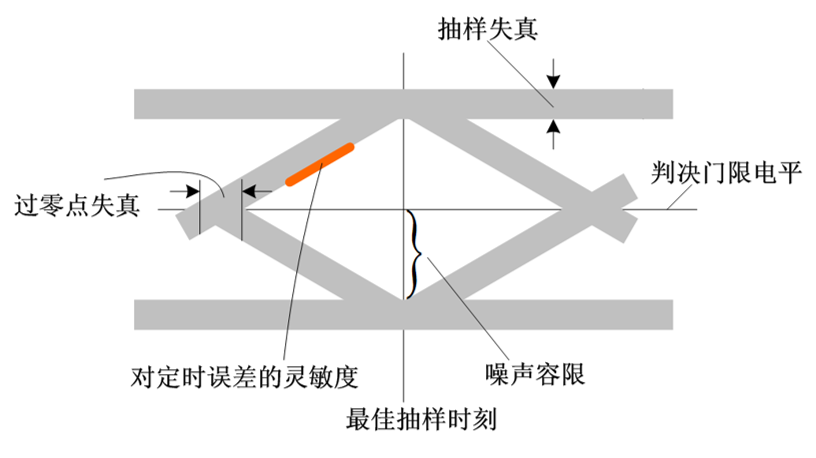
\includegraphics[width=0.7\textwidth]{eye.png}
\caption{眼图}
\end{figure}
\begin{itemize}
  \item 抽样最佳时刻是眼睛张开最大时刻
  \item 定时误差灵敏度是眼图斜边斜率 (越大越敏感)
  \item 中央横轴为判决门电平
  \item 最上方余辉高度, 表示抽样时刻上信号受到噪声干扰的畸变的程度
  \item 间隔距离的一半表示噪声容限 (若噪声瞬时值超过则可能会发生错判)
  \item 过零点畸变
\end{itemize}
M进制双极性波形, 在一个码周期$T_B$能看到$M-1$个眼睛. 
\section{部分响应}
人为, 有规律地在码元的抽样时刻引入ISI, 并在接收端判决前加以消除. 则可以改善频谱特性, 压缩传输频带, 使得频带利用率达到理论最大值. 把这种波形称为部分响应波形. 
(先引入ISI再消除)
\begin{figure}[H]
\centering
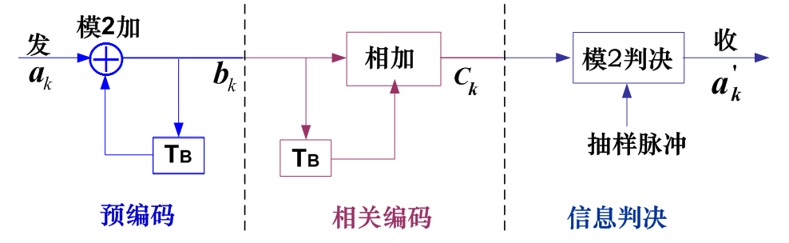
\includegraphics[width=0.7\textwidth]{partial_resp.png}
\caption{部分响应原理图}
\end{figure}
\begin{figure}[H]
\centering
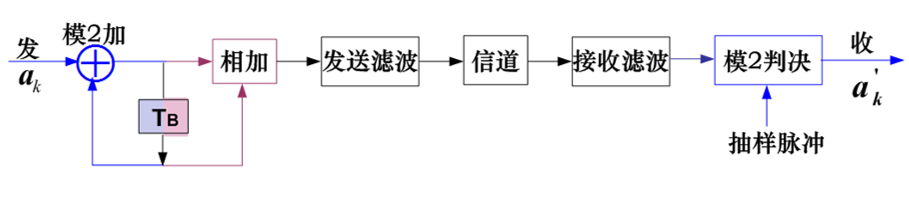
\includegraphics[width=0.7\textwidth]{partial_resp_sys.png}
\caption{部分响应系统图}
\end{figure}
感觉不会考计算题
\subsection{第I类部分响应波形}
两个sinc的叠加
\subsection{差错传播}
在恢复$a_k$时要参考$a_{k-1}$的值, 若有一项恢复错误则会影响之后所有项的正确判决. 
\subsection{相关编码}
这种串扰对应的运算称之为相关运算, 将\begin{equation}
  C_k=a_k+a_{k-1}
\end{equation}
称为相关编码
\subsection{预编码}
在相关编码之前进行预编码则可以避免差错传播. 

其实质就是把输入信码$a_k$变换成为差分码$b_k$, 差分的目的就是为了解除相关性. 
\begin{equation}
  b_k=a_k\oplus b_{k-1}
\end{equation}
或者
\begin{equation}
  a_k=b_k\oplus b_{k-1}
\end{equation}
$\oplus$为XOR, 或者模二加. 

完整过程为: 预编码$\Rightarrow$相关编码$\Rightarrow$模二判决. \\ 也就是已知$a_k,\; b_{k-1}$求$b_k$, 再由$b_k,\; b_{k-1}$求$C_k$
\section{时域均衡}
消除ISI的方式. 抽头横向滤波器. 利用自身产生的无限多个响应波形的和, 将接收滤波器输出端抽样时刻上有ISI的响应波形变换称为无ISI的. 
\begin{figure}[H]
\centering
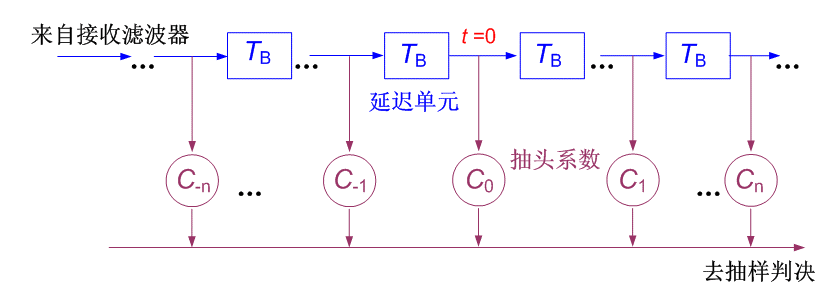
\includegraphics[width=0.7\textwidth]{transversal_filter.png}
\caption{横向滤波器}
\end{figure}
\begin{itemize}
  \item 横向滤波器的特性取决于各抽头系数
  \item 理论上, 无限长的横向滤波器可以完全消除抽样时刻上的ISI
\end{itemize}
设横向滤波器的抽头系数从$n$到$m$
\begin{equation}
  y_k=\displaystyle\sum_{i=n}^{m}C_i\cdot x_{k-i}
\end{equation}
\subsection{峰值失真}
均衡效果的衡量准则
\begin{equation}
  D=\frac{1}{y_0}\cdot \displaystyle\sum_{k=-\infty \; k\neq 0}^{\infty}\lvert y_k \rvert
\end{equation}
除了$k=0$以外, 各值的绝对值之和反应ISI的最大值. $D$越小越好. 
% \subsection{均方失真}
\subsection{迫零调整法}
题目会给一堆输入(若是三抽头就是$x_{-2}\sim x_{2}$); 可以列出如下矩阵
\begin{equation}
  \begin{bmatrix}
    x_0&x_{-1}&x_{-2}
    \\ x_1&x_{0}&x_{-1}
    \\ x_2&x_1&x_0
  \end{bmatrix}\cdot \begin{bmatrix}
    C_{-1}
    \\ C_0
    \\ C_1
  \end{bmatrix}=
  \begin{bmatrix}
    0
    \\ 1
    \\ 0
  \end{bmatrix}
\end{equation}
输入矩阵
\begin{equation}
  \begin{bmatrix}
    x_{t+1}&x_{t}\rvert_{\text{C对应时刻}}&x_{t-1}
  \end{bmatrix}
\end{equation}
令$C_0$输出为1, 其他输出为0. 输出有效范围就是$-3\sim 3$
\chapter{Digital Passband Modulation}
对应第七章, 数字带通传输系统; 第八章, 新型数字带通调制技术
\section{二进制分类}
\subsection{BASK}
OOK (On-off keying)
\begin{equation}
  e_{\text{BASK}}=s(t)\cdot \cos(\omega_c\cdot t)
\end{equation}
其中\begin{equation}
  s(t)=\displaystyle\sum_{n}a_n\cdot g(t-n\cdot T_B)
\end{equation}
$T_B$为码元的持续时间, $g(t)$为持续时间为$T_B$的基带脉冲波形, $a_n$是第$n$个符号的电平值, 对于二进制
\begin{equation}
  a_n=\begin{cases}
    1 &\text{概率为}P\\
    0 &\text{概率为}1-P
  \end{cases}
\end{equation}
产生方法\begin{itemize}
  \item 乘法器法(模拟调制法)
  \item 键控法
\end{itemize}
解调方法\begin{itemize}
  \item 非相干解调 (包络检波)
  \item 相干解调 (同步检波)
\end{itemize}
\subsubsection{非相干解调}
\begin{figure}[H]
\centering
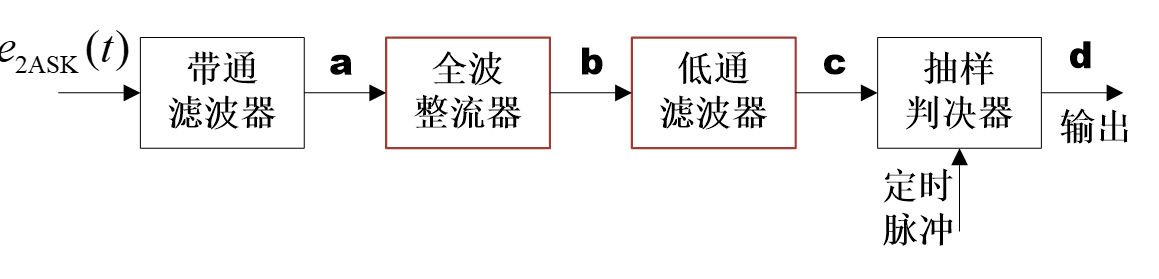
\includegraphics[width=0.7\textwidth]{bask_non_co.png}
\caption{BASK非相干解调框图}
\end{figure}
\begin{figure}[H]
\centering
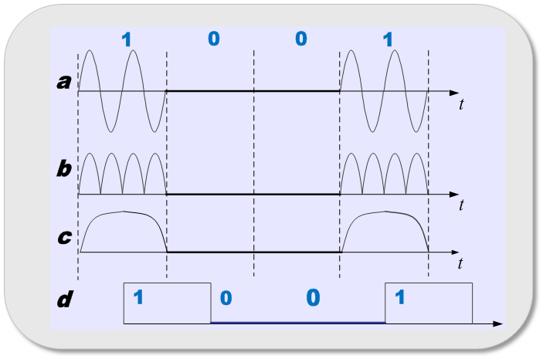
\includegraphics[width=0.7\textwidth]{bask_non_co_wave.png}
\caption{BASK非相干解调波形}
\end{figure}

抽样判决后的输出要延后一些(半个周期), 绝对不可以对齐. 
\subsubsection{相干解调}
BPF之后乘上同频率的载波(乘法器), 再过LPF之后判决
\begin{figure}[H]
\centering
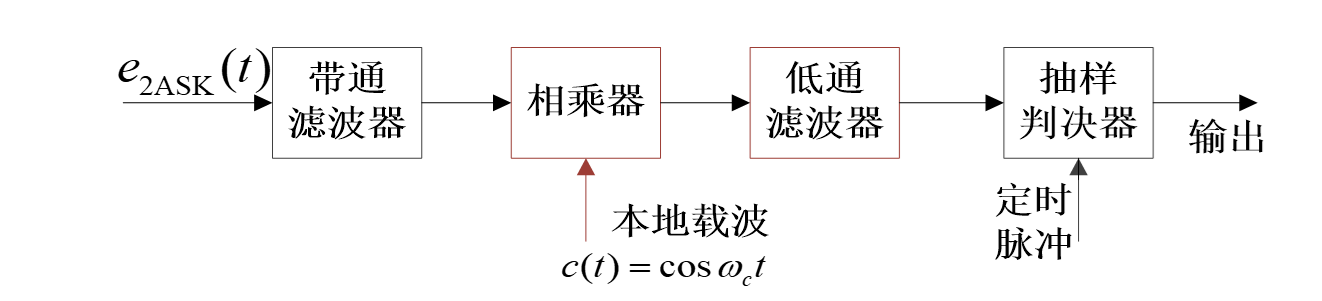
\includegraphics[width=0.8\textwidth]{bask_co.png}
\caption{BASK相干解调}
\end{figure}
\subsubsection{功率谱密度}
\begin{equation}
  P_{\text{BASK}}(f)=\frac{1}{4}\cdot [P_s(f+f_c)+P_s(f-f_c)]
\end{equation}
其中$P_s(f)$为单极性基带信号功率谱. \\$P_s$左移, 右移, 再带直流分量
\subsubsection{带宽}
\begin{equation}
  B_{BASK}=2\cdot f_B
\end{equation}
频带利用率
\begin{equation}
\eta=\frac{R_B}{B}
\end{equation}
单位为 bit/(s$\cdot$Hz) (bps/Hz)

$f_B=\frac{1}{T_B}=R_B$为基带信号带宽(码元速率)的两倍
\subsection{BFSK}
\begin{equation}
  e_{\text{BFSK}}=s_1(t)\cdot \cos(\omega_1\cdot t)+s_2(t)\cdot\cos(\omega_2\cdot t)
\end{equation}
其中
$$\begin{cases}
  s_1(t)=\text{正电平 (1)}
  \\   s_2(t)=\text{零电平 (0)}
\end{cases}$$

\begin{figure}[H]
\centering
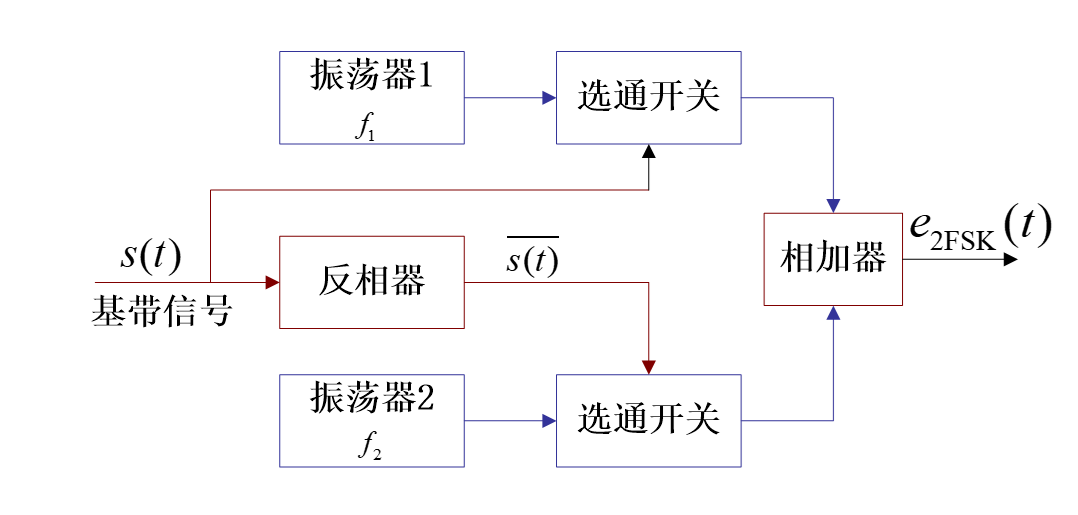
\includegraphics[width=0.5\textwidth]{bfsk_keying.png}
\caption{BFSK键控法调制}
\end{figure}

解调方法
\begin{itemize}
  \item 非相干解调 (俩包络检波)
  \item 相干解调 (俩乘法器) 最好用相干解调啦
  \item 过零检测
\end{itemize}

\begin{figure}[H]
\centering
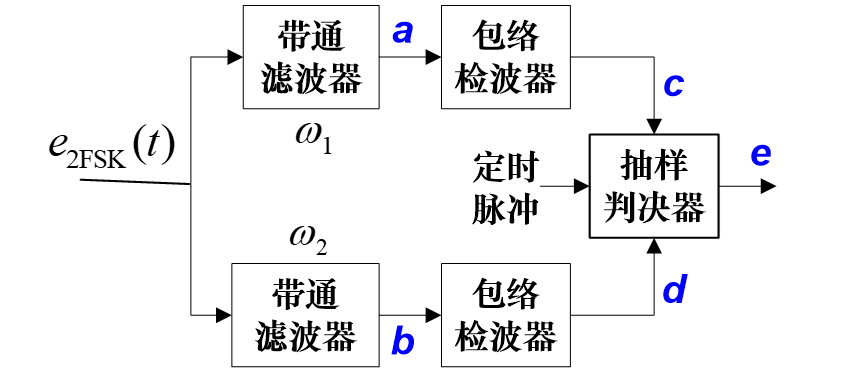
\includegraphics[width=0.7\textwidth]{bfsk_non_co.png}
\caption{BFSK非相干解调}
\end{figure}

\begin{figure}[H]
\centering
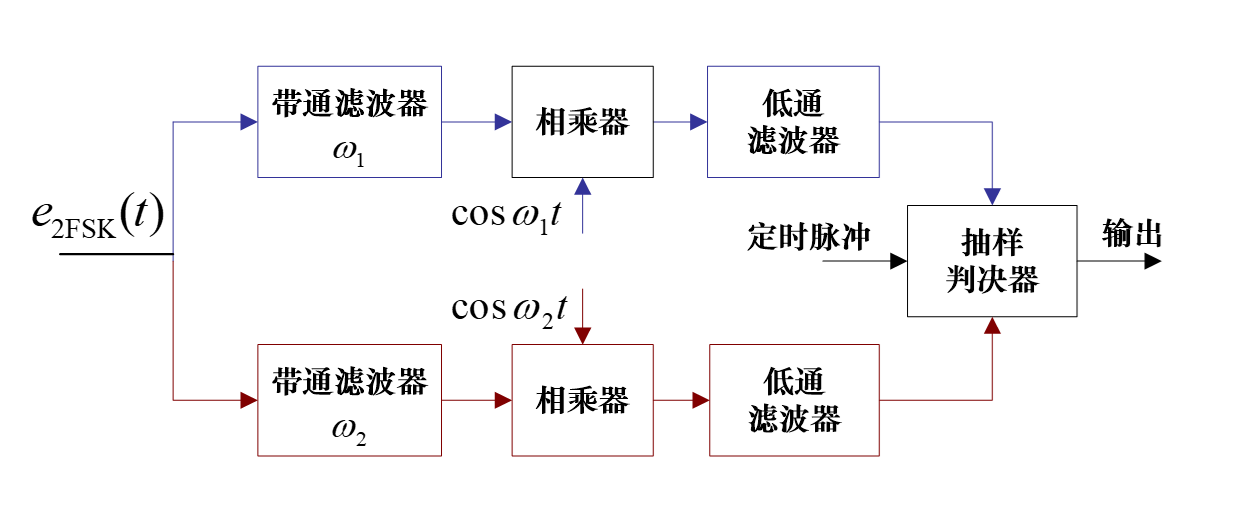
\includegraphics[width=0.7\textwidth]{bfsk_co.png}
\caption{BFSK相干解调}
\end{figure}


\subsubsection{过零检测法}
限幅(信号变为方波), 微分(上升沿变上脉冲, 下降沿变下脉冲), 整流(单极性脉冲), 脉冲展宽(一堆频率不同的方波), LPF(根据脉冲展宽之后的不同方波频率来滤波). 

\begin{figure}[H]
\centering
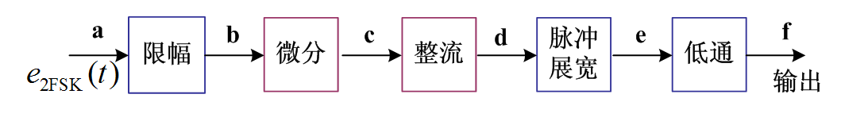
\includegraphics[width=0.7\textwidth]{bfsk_zero_crossing.png}
\caption{BFSK过零检测法框图}
\end{figure}
\begin{figure}[H]
\centering
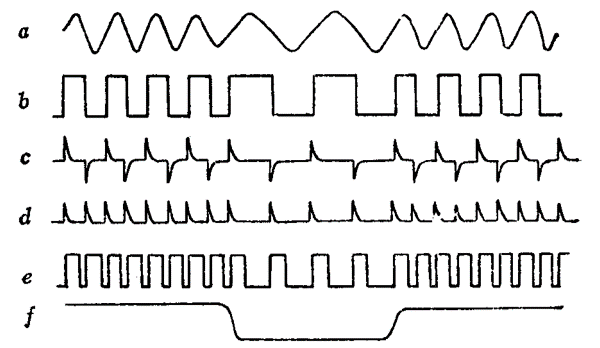
\includegraphics[width=0.7\textwidth]{bfsk_zero_crossing_wave.png}
\caption{BFSK过零解调波形}
\end{figure}

\subsubsection{带宽}
\begin{equation}
  B_{\text{BFSK}}=\lvert f_2 - f_1 \rvert +2\cdot f_B
\end{equation}
$f_B=\frac{1}{T_B}=R_B$
\subsubsection{功率谱密度}
\begin{equation}
  P_{\text{BFSK}}(f)=\frac{1}{4}\cdot [P_{s1}(f+f_1)+P_{s1}(f-f_1)]+\frac{1}{4}\cdot [P_{s2}(f+f_2)+P_{s2}(f-f_2)]
\end{equation}
是两组BASK的功率谱密度的叠加
\begin{itemize}
  \item 若$\lvert f_2 - f_1 \rvert <f_B$, 功率谱再$f_0$处有单峰
  \item 若$\lvert f_2 - f_1 \rvert >f_B$, 功率谱再$f_0$处有双峰
\end{itemize}
直流分量(离散谱), 即箭头仍然存在, 是功率谱密度的组成部分. 
\subsection{BPSK}
\begin{equation}
  e_{\text{BPSK}}=s(t)\cdot \cos(\omega_c\cdot t)
\end{equation}

其中\begin{align*}
  s(t)=\displaystyle\sum_{n}a_n\cdot g(t-n\cdot T_B)
\end{align*}
$T_B$为码元的持续时间, $g(t)$为持续时间为$T_B$的基带脉冲波形, $a_n$是第$n$个符号的电平值, 对于二进制
\begin{equation}
  a_n=\begin{cases}
    1 &\text{概率为}P\\
    -1 &\text{概率为}1-P
  \end{cases}
\end{equation}
也就是用0和$\pi$

向左挪$\frac{1}{2}$个码元周期 (半个码元周期$T_B$) 或者说偶对称来对称下. 

只能采用相干解调. 
\subsubsection{相干解调}
与载波同相, 乘法器出来是向上的尖顶余弦脉冲; 反向, 乘法器出来是向下的尖顶余弦脉冲. 
\begin{figure}[H]
\centering
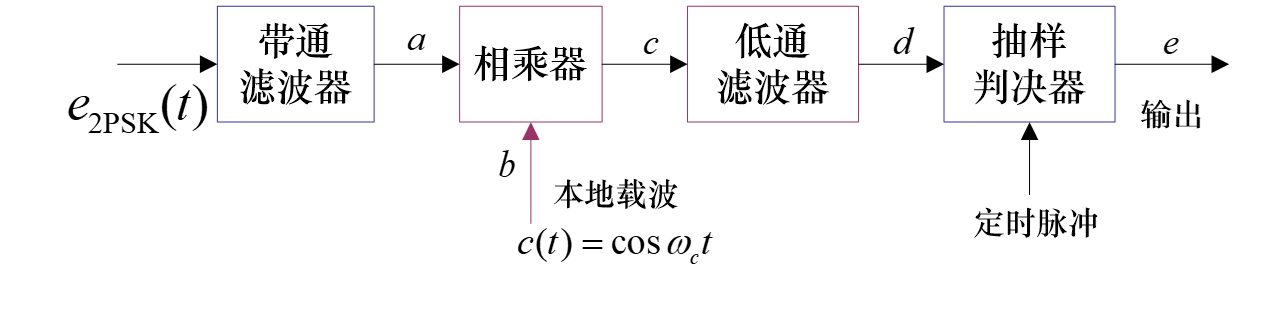
\includegraphics[width=0.7\textwidth]{bpsk_co.png}
\caption{BPSK相干解调}
\end{figure}

\begin{figure}[H]
\centering
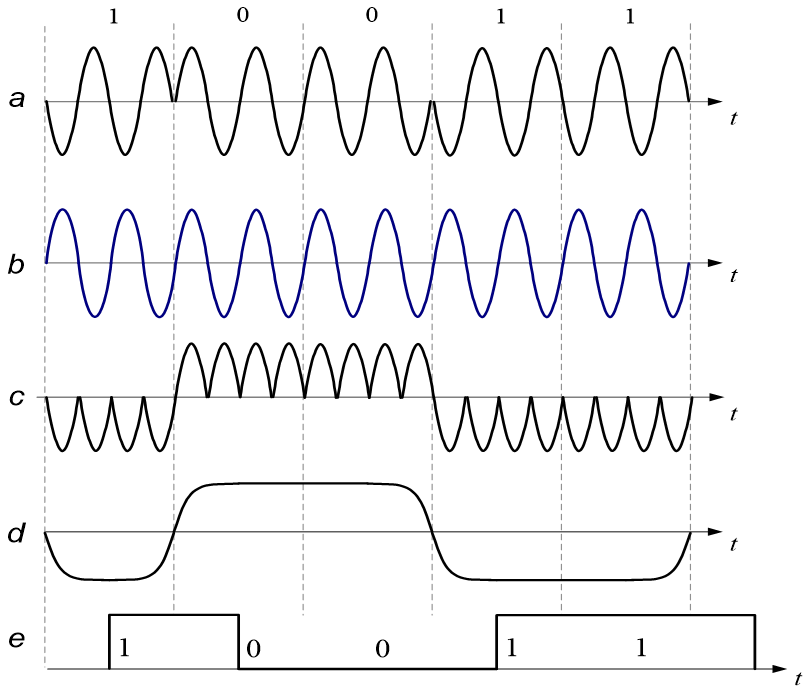
\includegraphics[width=0.7\textwidth]{bpsk_co_wave.png}
\caption{BPSK相干解调波形}
\end{figure}

\subsubsection{带宽和功率谱密度}
参照BASK
\subsection{BDPSK}
前后码元相对的相位差才唯一决定信息符号. 必须规定首位码元的相位. 

与前一码元的相位相同为0, 不相同为1. 
\begin{itemize}
  \item 相干解调 (极性比较法)
  \item 差分相干解调 (非相干解调) (相位比较法)
\end{itemize}
\subsubsection{相干解调}
与载波同相, 乘法器出来是向上的尖顶余弦脉冲; 反向, 乘法器出来是向下的尖顶余弦脉冲. 得到相对码. 

\begin{figure}[H]
\centering
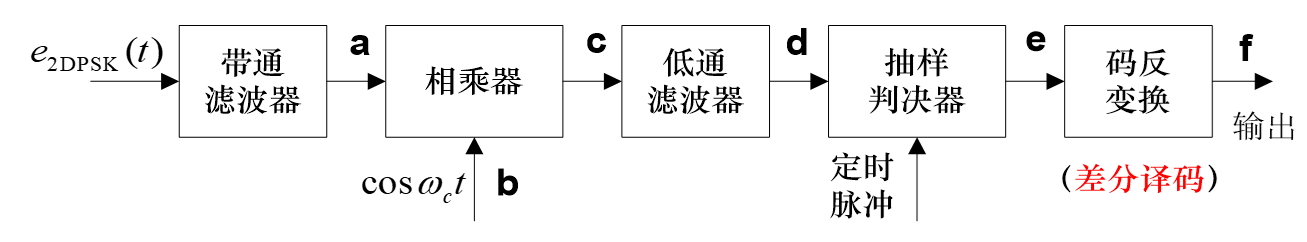
\includegraphics[width=0.7\textwidth]{bdpsk_co.png}
\caption{BDPSK相干解调}
\end{figure}

\begin{figure}[H]
\centering
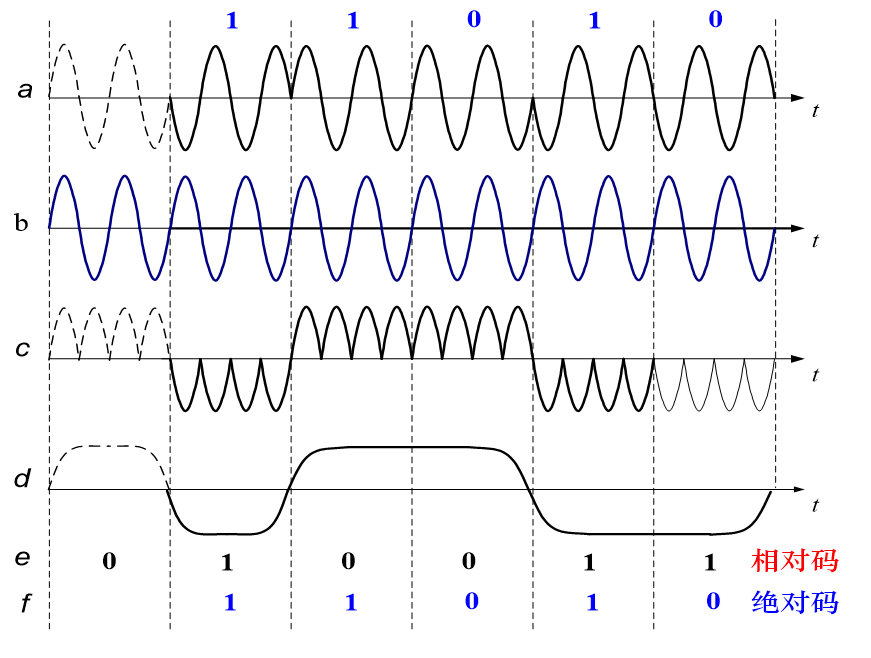
\includegraphics[width=0.7\textwidth]{bdpsk_co_wave.png}
\caption{BDPSK相干解调波形}
\end{figure}
相对码与绝对码之间转换. 

\subsubsection{差分相干解调}
不用本地载波, 而是与延时一周期的自身信号相乘. 故为非相干解调. 
\begin{figure}[H]
\centering
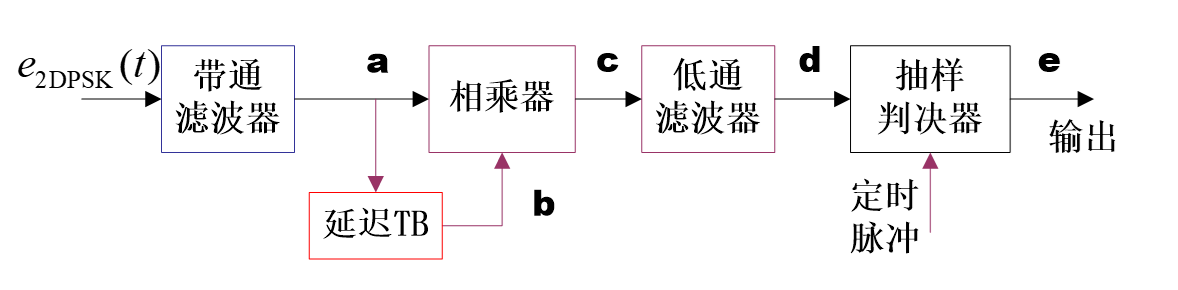
\includegraphics[width=0.7\textwidth]{bdpsk_non_co.png}
\caption{BDPSK差分相干解调}
\end{figure}

\begin{figure}[H]
\centering
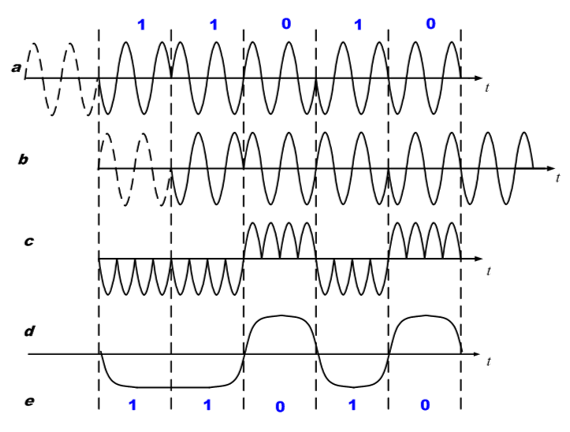
\includegraphics[width=0.7\textwidth]{bdpsk_non_co_wave.png}
\caption{BDPSK差分相干解调波形}
\end{figure}

可以直接得到绝对码. 
\subsubsection{带宽和功率谱密度}
和BPSK, BASK相同. 
\section{码元周期和载波周期}
已知码元率为2000 Baud. 载波为$\sin(8\pi\times 10^3\cdot t)$. 求每个码元包含多少个载波周期. 

二进制, 比特率等于波特率. 每个码元包含的载波周期, 也就是拿$T_B$去比上$T_\omega$
\begin{align*}
  \omega&=8\pi\cdot 10^3\\
  T_\omega&=\frac{1}{f}=\frac{2\pi}{\omega}
  \\ &=\frac{2\pi}{8\pi\cdot 10^3}
  \\ &=\frac{1}{4000}
  \\ T_B&=\frac{1}{R_B}=\frac{1}{2000}
  \\ \frac{T_B}{T_\omega}&=2
\end{align*}
\section{二进制带通调制性能分析}
\subsection{可靠性}
误码率代表着可靠性, 代表着方式抗噪声性能的强弱. 
% Table generated by Excel2LaTeX from sheet 'Sheet1'
\begin{table}[H]
  \centering
    \begin{tabular}{|c|cc|c}
    \multirow{2}[0]{*}{调制方式} & \multicolumn{2}{c}{相干解调} & \multirow{2}[0]{*}{非相干解调} \\
          & 精确    & 近似    &  \\
    BASK  &    $\frac{1}{2}\text{erfc}(\sqrt{\frac{r}{4}})$   &   $\frac{1}{\sqrt{\pi r}}\cdot e^{-\frac{r}{4}}$    & $\frac{1}{2}\cdot e^{-\frac{r}{4}}$ \\
    BFSK  &    $\frac{1}{2}\text{erfc}(\sqrt{\frac{r}{2}})$   &   $\frac{1}{\sqrt{2\pi r}}\cdot e^{-\frac{r}{2}}$    &  $\frac{1}{2}\cdot e^{-\frac{r}{2}}$\\
    BPSK  &    $\frac{1}{2}\text{erfc}(\sqrt{r})$   &   $\frac{1}{2\sqrt{\pi r}}\cdot e^{-r}$    & N/A \\
    BDPSK &    $\text{erfc}(\sqrt{r})$   &    $\frac{1}{\sqrt{\pi r}}\cdot e^{-r}$   & $\frac{1}{2}\cdot e^{-r}$ \\
    \end{tabular}%
  \caption{各调制方式误码率表}
\end{table}%
\begin{itemize}
  \item $r$一定, 相同调制方式, 抗AWGN的性能优劣顺序\footnote{$P_e$越小越好; erfc为单调递减函数, 也就是说erfc的参数取值越小误码率越大, 性能越差}: 2PSK, 2DPSK, 2FSK, 2ASK
  \item $P_e$一定, 所需要的信噪比$r$: $r_\text{BASK}=2r_\text{BFSK}=4r_\text{BPSK}$ (若用dB来作为信噪比的话, 递增3dB)
  \item $r$一定, 相同调制方式: 相干解调信噪比总是会小一些的; 但是在大信噪比时两者相差不大. 
\end{itemize}


\paragraph{具体例子}
以BASK相干解调为例进行说明
最佳判决门限
\begin{equation}
  b^*=\frac{a}{2}+\frac{\sigma^2_n}{a}\cdot \ln{\frac{P(0)}{P(1)}}
\end{equation}
当等概时
\begin{equation}
  b^*=\frac{a}{2}
\end{equation}
误码率
\begin{equation}
  P_e=\frac{1}{2}\cdot \text{erfc}(\sqrt{\frac{r}{4}})
\end{equation}
其中
\begin{equation}
  r=\frac{a^2}{2\cdot \sigma^2_n}
\end{equation}
信号功率为$\frac{a^2}{2}$, 噪声功率为$\sigma^2_n=n_0\cdot B$

% 大信噪比时
% \begin{equation}
%   P_e\approx \frac{1}{\sqrt{\pi\cdot r}}\cdot e^{-\frac{r}{4}}
% \end{equation}
% \subsubsection{包络检波}
% \begin{equation}
%   P_e=\frac{1}{2}\cdot e^{-\frac{r}{4}}
% \end{equation}
\subsection{有效性}
设基带信号的谱零点带宽为$R_B=\frac{1}{T_s}$
\begin{equation}
  B_{\text{BASK}}=B_{\text{BPSK}}=B_{\text{BDPSK}}=2\cdot R_B=\frac{2}{T_s}
\end{equation}
\begin{equation}
  B_{\text{BFSK}}=\lvert f_2 -f_1\rvert+2\cdot R_B
\end{equation}
在$R_B$一定时, BFSK的频带利用率最低. 
\subsection{判决门限}
\begin{itemize}
  \item BASK: $b^*=\frac{a}{2}$ 易受信道参数变换的影响
  \item BFSK: 不需要人为设置判决门限, 对信道的变换不敏感
  \item BPSK: $b^*=0$ (等概时) 不易受信道参数变换的影响
\end{itemize}



\section{多进制}
多进制码元进制数为$M$, 
信息比特数\begin{equation}
  k=\log_2{M}
\end{equation}
把信号功率$\frac{a^2}{2}$均分为$k$个bit
\begin{equation}
  P_b=\frac{a^2}{2\cdot k}
\end{equation}
故有每比特信噪比
\begin{equation}
  r_b=\frac{a^2}{2k\cdot \sigma^2_n}=\frac{r}{k}
\end{equation}
\subsection{MASK}
带宽利用率超过 1 bit/s $\cdot$ Hz

基带的带宽利用率为 2 bit/s Hz
\subsection{MFSK}
\begin{equation}
  B=f_{H}-f_L+\Delta f
\end{equation}
$\Delta f$为单个码元变换带宽, $f_H,\; f_L$分别为最高频和最低频
\subsection{MPSK}
均匀间隔时的受调制相位
\begin{equation}
  \theta_k=\frac{2\pi}{M}\cdot (k-1)\qquad k=1,2\dots M
\end{equation}
\subsection{QPSK}
\subsubsection{A方式}
格雷码: 相邻相位的两bit只有一个bit不相同
\begin{itemize}
  \item 00: 90
  \item 11: 270
  \item 10: 180
  \item 01: 0
\end{itemize}
产生方法
\begin{itemize}
  \item 正交调相法
  \item 相位选择法
\end{itemize}
\subsubsection{B方式}
A方式转45度, 像个叉叉. 
\subsection{MDPSK}
相对于前一码元的相位变化. $\theta_k$当作是相对于前一码元相位的相移

B方式$$\Delta \theta_k=45,135,225,315 \; \text{deg}$$
\section{多进制误码率}
\subsection{MASK}
\begin{equation}
  P_e=(1-\frac{1}{M})\cdot \text{erfc}(\sqrt{\frac{3}{M^2-1}\cdot r})
\end{equation}
其中\begin{equation}
  r=\frac{P_s}{\sigma_n^2}
\end{equation}为信噪比. 而$M$为电平数
\subsection{MFSK}
有上界(最差的值)

当进制数$k>7$时, 相干与非相干均写成
\begin{equation}
  P_e\leq \frac{M-1}{2}\cdot e^{-\frac{r^2}{\sigma_n^2}}
\end{equation}
\subsection{QPSK}
四进制
\begin{equation}
  P_e=1-[1-\frac{1}{2}\cdot \text{erfc}(\sqrt{\frac{r}{2}})]^2
\end{equation}
\subsection{MPSK}
$M$进制
\begin{equation}
  P_e=\text{erfc}(\sqrt{r}\cdot\sin{\frac{\pi}{M}})
\end{equation}
\subsection{MDPSK}
\begin{equation}
  P_e\approx \text{erfc}(\sqrt{2 r}\cdot \sin{\frac{\pi}{2M}})
\end{equation}

\section{新型数字基带}
\subsection{Quadrature Amplitude Modulation}
正交振幅调制, 一种把振幅(ASK)和相位(PSK)结合起来的调制方式. 

星座图
\subsection{最小频移键控}
MSK(Minimum-Shift Keying)就是一种包络恒定, 相位连续, 频差最小并且严格正交的2FSK信号
\begin{itemize}
  \item 振幅恒定
  \item 频偏严格等于$\pm\frac{1}{4T_B}$
  \item 在一个码元周期内以载波相位为基准的信号相位准确变换$\pm\frac{\pi}{2}$
  \item 信号的相位在码元转换时刻是连续的
\end{itemize}
\subsubsection{附加相位路径图}
\begin{figure}[H]
\centering
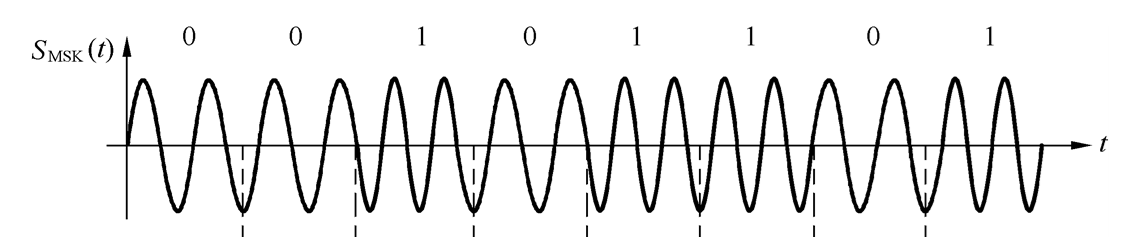
\includegraphics[width=0.7\textwidth]{msk_wave.png}
\caption{MSK波形信号}
\end{figure}
在码元转换时刻, MSK的相位是连续的. 
\begin{figure}[H]
\centering
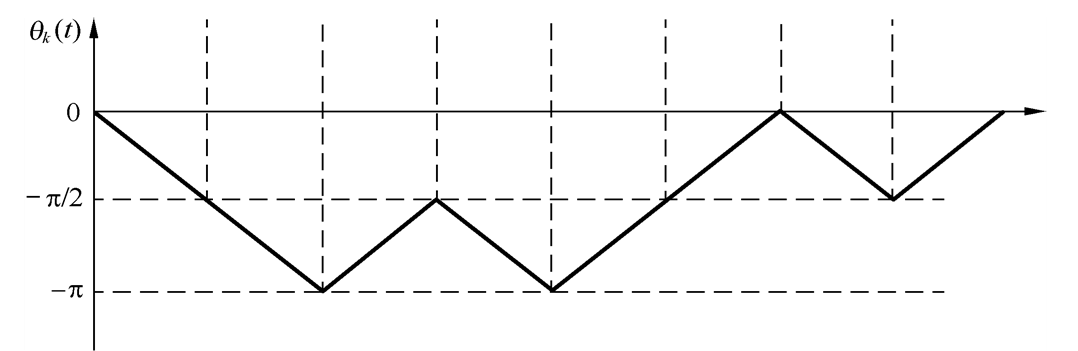
\includegraphics[width=0.7\textwidth]{msk_phase.png}
\caption{MSK附加相位路径图}
\end{figure}


设接收电压$r(t)$
\begin{equation}
  r(t)=s(t)+n(t)
\end{equation}
发送码元确定后, 接收电压$r(t)$的随机性完全由噪声决定, 服从高斯分布, 其方差为$\sigma_n^2$, 均值为$s(t)$

发送码元「0」的信号波形为$s_0(t)$时, 接收电压$r(t)$的$k$维联合概率密度函数为
\begin{align*}
  f_0(\vec{r})=\frac{1}{(\sqrt{2\pi}\cdot \sigma_n)^k}\cdot \exp \Bigg( - \frac{1}{n_0}\int_0^{T_B} [r(t)-s_0(t)]^2 \;\text{d}t \Bigg)
\end{align*}
式中$\vec{r}=\vec{s}+\vec{n}$, 表示一个码元内接收电压的$k$个抽样值. 

\chapter{Optimum Receiver}
\section{确知信号的最佳接收机}
$W$为加权因子
\begin{align}
  W_1+\int_0^{T_B} r(t)\cdot s_1(t) \; \text{d}t<
  W_0+\int_0^{T_B} r(t)\cdot s_0(t) \; \text{d}t
\end{align}
则判为$s_0(t)$, 否则判为$s_1(t)$


当先验概率$P(0)=P(1)=\frac{1}{2}$时
\begin{align}
  \int_0^{T_B} r(t)\cdot s_1(t) \; \text{d}t<
  \int_0^{T_B} r(t)\cdot s_0(t) \; \text{d}t
\end{align}
则判为$s_0(t)$, 否则判为$s_1(t)$
\begin{figure}[H]
\centering
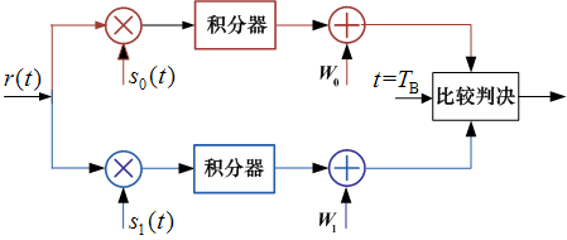
\includegraphics[width=0.7\textwidth]{opt_rx_1.png}
\caption{最佳接收机}
\end{figure}
\begin{figure}[H]
\centering
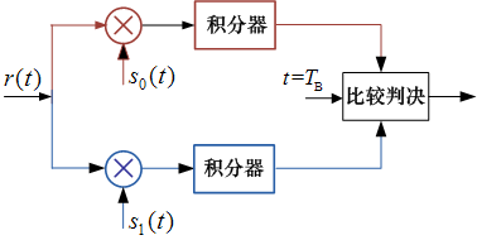
\includegraphics[width=0.7\textwidth]{opt_rx_2.png}
\caption{最佳接收机(等概)}
\end{figure}
\begin{figure}[H]
\centering
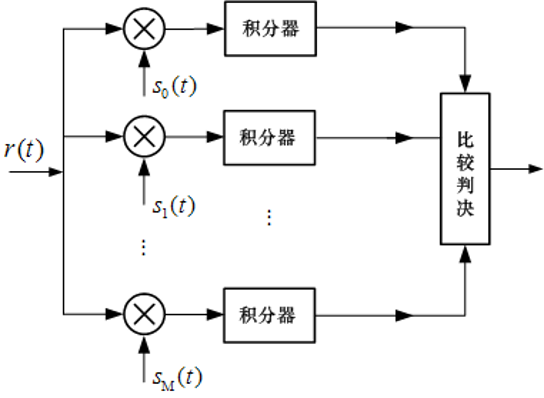
\includegraphics[width=0.7\textwidth]{opt_rx_3.png}
\caption{最佳接收机(等概M进制)}
\end{figure}
\subsection{误码率}
$E_b$为码元能量, $\rho$为码元相关系数, $n_0$为噪声单边功率谱密度
\begin{equation}
  P_e=\frac{1}{2}\cdot \text{erfc}\bigg(\sqrt{\frac{E_b\cdot (1-\rho)}{2n_0}}\bigg)
\end{equation}

误码率仅与$\frac{E_b}{n_0}=\frac{P_s}{P_n}$和相关系数$\rho$有关. 与信号波形和噪声功率无直接关系. 
\subsubsection{相关系数}
\begin{itemize}
  \item $\rho=1$时, 两种码元波形相同, 相关系数最大, $P_e=\frac{1}{2}$ (最差情况, 瞎鸡巴猜)
  \item $\rho=-1$时, 两种码元的波形相反, 如2PSK, $  P_e=\frac{1}{2}\cdot \text{erfc}\big(\sqrt{\frac{E_b}{n_0}}\big)$
  \item $\rho=0$时, 两者码元波形正交, 如2FSK, $  P_e=\frac{1}{2}\cdot \text{erfc}\big(\sqrt{\frac{E_b}{2n_0}}\big)$
  \item 当其中有一码元为0时, $\rho=\frac{1}{2}$, 如2ASK, $  P_e=\frac{1}{2}\cdot \text{erfc}\big(\sqrt{\frac{E_b}{4n_0}}\big)$, 有$E_0=0,\; E_1=E_b$
\end{itemize}

2ASK信号的性能比2FSK信号的性能差3dB, 2FSK比2PSK又差3dB. 

\subsubsection{码元能量}
\begin{equation}
  E_b=\int_0^{T_B} s^2(t)\; \text{d}t
\end{equation}
一般来说$E_1=E_0=E_b$

还有一种求码元能量$E_b$的方式, 若$B=\frac{1}{T_B}$ (不一定成立), 则有
\begin{equation}
  \frac{E_b}{n_0}=\frac{P_s}{B\cdot n_0}=\frac{P_s}{P_n}
\end{equation}
M进制中包含的比特数为$\log_2{M}$, 故每比特的能量为$E_b=\frac{E}{\log_2{M}}$, 每比特的信噪比为$\frac{E_b}{n_0}=\frac{E}{n_0\cdot \log_2{M}}$
\section{实际接收机和最佳接收机的性能比较}
最佳接收机的误码率就是把实际接收机的误码率公式之中的$r$换成$\frac{E_b}{n_0}$就完事了

以BPSK为例
\begin{align*}
  P_e=\frac{1}{2}\text{erfc}(\sqrt{\frac{E_b}{n_0}})\\
  P_e=\frac{1}{2}\text{erfc}(\sqrt{r})
\end{align*}
那么$r$和$\frac{E_b}{n_0}$有啥关系呢
\begin{align*}
  r&=\frac{P_s}{P_n}
  \\ &=\frac{\frac{a^2}{2}}{\sigma_n^2}
  \\ &=\frac{\frac{E_b}{T_B}}{n_0\cdot B}
\end{align*}
其中$\frac{a^2}{2}$为信号功率, $\sigma_n^2=n_0\cdot B$为噪声功率; 但信号功率$P_s$也等于$\frac{E_b}{T_B}$也就是码元能量乘上码元间隔. 

若$B=\frac{1}{T_B}$则
\begin{align*}
  r=\frac{E_b}{n_0}
\end{align*}
但是一般来说$B>\frac{1}{T_B}$

\end{document}